% CVPR 2022 Paper Template
% based on the CVPR template provided by Ming-Ming Cheng (https://github.com/MCG-NKU/CVPR_Template)
% modified and extended by Stefan Roth (stefan.roth@NOSPAMtu-darmstadt.de)
%
% Compile with: xelatex (required for xeCJK / Noto Serif CJK TC).

\documentclass[10pt,twocolumn,letterpaper]{article}

%%%%%%%%% PAPER TYPE  - PLEASE UPDATE FOR FINAL VERSION
% \usepackage[review]{cvpr}      % To produce the REVIEW version
% \usepackage{cvpr}              % To produce the CAMERA-READY version
\usepackage[pagenumbers]{cvpr} % To force page numbers, e.g. for an arXiv version

% Include other packages here, before hyperref.
\usepackage{subcaption}
\usepackage{graphicx}
\usepackage{amsmath}
\usepackage{amssymb}
\usepackage{booktabs}
\usepackage{array}
\usepackage{pgffor}
\usepackage[dvipsnames]{xcolor}
\usepackage[newfloat]{minted}
\usepackage[breakable, listings, skins, minted]{tcolorbox}
\setminted{fontsize=\footnotesize}
\renewtcblisting{minted}{%
    listing engine=minted,
    minted language=python,
    listing only,
    breakable,
    enhanced,
    minted options = {
        linenos,
        breaklines=true,
        breakbefore=.,
        numbersep=2mm
    },
    overlay={%
        \begin{tcbclipinterior}
            \fill[gray!25] (frame.south west) rectangle ([xshift=4mm]frame.north west);
        \end{tcbclipinterior}
    }
}
\usepackage{xeCJK}
\setCJKmainfont{Noto Serif CJK TC}

\usepackage[pagebackref,breaklinks,colorlinks]{hyperref}

% Support for easy cross-referencing
\usepackage[capitalize]{cleveref}
\crefname{section}{Sec.}{Secs.}
\Crefname{section}{Section}{Sections}
\Crefname{table}{Table}{Tables}
\crefname{table}{Tab.}{Tabs.}

\begin{document}

%%%%%%%%% TITLE
\title{\LARGE Lab4 Conditional VAE for Video Prediction Report \\[0.5em] \large Deep Learning, NYCU}
\author{朱驛庭, 111550093}
\maketitle

%%%%%%%%% BODY TEXT
\section{Introduction}
\label{sec:intro}

In this lab we implement a \textbf{conditional variational autoencoder (cVAE)} for pose-conditioned video prediction. Given a single past frame $x_1$ and a sequence of pose images $\{P_2,\ldots,P_T\}$, the model autoregressively generates the remaining $T{-}1$ frames. The architecture follows the standard cVAE protocol (\cref{fig:arch}) and draws on two standard references: \emph{Everybody Dance Now}~\cite{chan2019everybody} for the pose-conditioned generation idea, and \emph{Stochastic Video Generation with a Learned Prior}~\cite{denton2018svg} for the VAE-based latent-variable formulation.

The key training challenge is the well-known \textbf{KL-vanishing} problem of VAEs combined with \textbf{exposure bias} of autoregressive sequence models. We address both with: (i) cyclical / monotonic KL annealing~\cite{fu2019cyclical}; (ii) a teacher-forcing schedule that gradually transitions the decoder from ground-truth conditioning to its own predictions; and (iii) a numerically stable KL criterion with logvar clamping and proper element-wise normalization. Our final model (Monotonic annealing, fixed pipeline) reaches a per-frame validation \textbf{PSNR of 38.87~dB} averaged over the 629 predicted frames. Our extended-training submission (Cyclical, 140 epochs) achieved \textbf{PSNR 35.84164 on the Kaggle public leaderboard, ranked 19th}.

The report is organized as follows: \cref{sec:implement} describes the model, the training/testing protocol, and our concrete choices for the reparameterization trick, teacher forcing, and KL annealing. \cref{sec:exp} compares the three KL annealing strategies, dissects the teacher-forcing schedule, presents the per-frame PSNR analysis, and discusses the bug-fix that took us from a collapsed PSNR$\approx$19~dB run to PSNR$\approx$38~dB.

\begin{figure*}[t]
    \centering
    \begin{subfigure}[b]{0.62\linewidth}
        \centering
        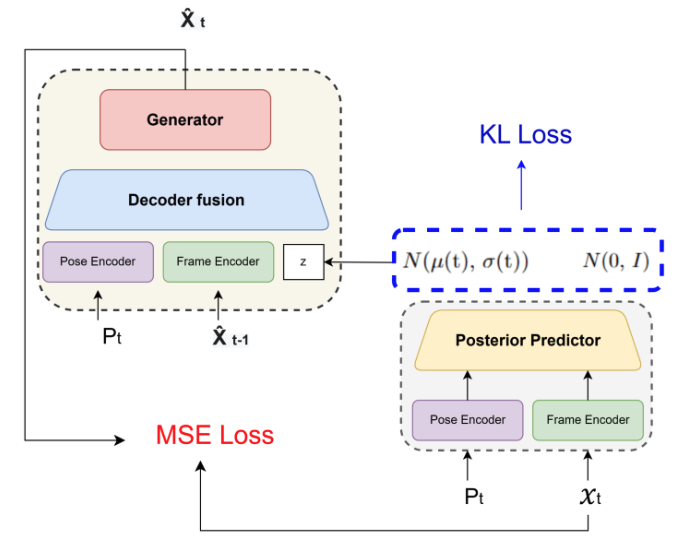
\includegraphics[height=5.4cm,keepaspectratio]{assets/arch_train.png}
        \caption{\textbf{Training.} Posterior Predictor takes the ground-truth current frame $x_t$ and pose $P_t$ and outputs $\mathcal{N}(\mu_t, \sigma_t^2)$, regularized toward $\mathcal{N}(0, I)$ via the KL loss. Sampled $z_t$ together with the encoded previous frame $\hat{x}_{t-1}$ and pose $P_t$ are fused and decoded into $\hat{x}_t$, supervised by MSE against $x_t$.}
        \label{fig:arch_train}
    \end{subfigure}
    \hfill
    \begin{subfigure}[b]{0.34\linewidth}
        \centering
        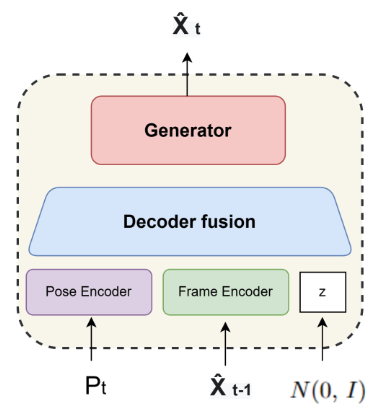
\includegraphics[height=5.4cm,keepaspectratio]{assets/arch_inference.png}
        \caption{\textbf{Inference.} The posterior is dropped: $z \sim \mathcal{N}(0, I)$ is sampled from the prior. Only $\hat{x}_{t-1}$ and $P_t$ condition the prediction, fed back autoregressively for the full 629-frame rollout.}
        \label{fig:arch_inference}
    \end{subfigure}
    \caption{\textbf{Conditional VAE pipeline.} (a) Training uses the posterior network on $(x_t, P_t)$ to produce a tight latent distribution; reconstruction is supervised by MSE and regularized by KL. (b) At inference time, the posterior is unavailable so $z$ is sampled from the prior; predictions feed back autoregressively. Diagrams reproduced from the lab specification.}
    \label{fig:arch}
\end{figure*}

%------------------------------------------------------------------------
\section{Implementation Details} \label{sec:implement}

\subsection{Model Overview}

The five modules in \texttt{src/modules/} are kept structurally unchanged per the spec. They are wired together in \texttt{Trainer.py} as illustrated in \cref{fig:arch}. Let $F\!=\!128, L\!=\!32, N\!=\!12, D_{out}\!=\!192$ denote the feature dimensions of the frame encoder, label encoder, latent, and decoder fusion output respectively, and $H\!\times\!W = 32\!\times\!64$ the resized frame size.

\begin{itemize}
    \item \textbf{Frame Encoder} (\texttt{RGB\_Encoder}): RGB frame $\to$ $F$-channel feature.
    \item \textbf{Pose Encoder} (\texttt{Label\_Encoder}): pose image $\to$ $L$-channel feature.
    \item \textbf{Posterior Predictor} (\texttt{Gaussian\_Predictor}): consumes the encoded current frame and current pose and outputs $(\mu,\log\sigma^2)$ of dimension $N$ at the spatial size of the encoder.
    \item \textbf{Decoder Fusion} (\texttt{Decoder\_Fusion}): concatenates the encoded \emph{previous} frame, the encoded current pose, and the sampled latent $z$, then projects to $D_{out}$ channels.
    \item \textbf{Generator}: $D_{out}$-channel feature $\to$ RGB image.
\end{itemize}

\subsection{Training / Testing Protocol}

\paragraph{Training.} Each training clip contains $T{=}16$ frames and 16 paired pose maps. We unroll the model frame-by-frame; at each step $t \in \{1,\ldots,T-1\}$ the network sees the encoded previous frame, the encoded next pose $P_{t+1}$, and a latent $z_t \sim \mathcal{N}(\mu_t, \sigma_t^2)$ sampled by the \emph{posterior} predictor (which gets to look at the ground-truth next frame $x_{t+1}$). The previous frame fed to the decoder is either the ground-truth $x_t$ (\emph{teacher forcing}) or the model's own previous output $\hat x_t$, decided by a Bernoulli draw with probability $\rho_{tf}$ (per-batch). The per-clip loss is the time-summed VAE objective
\begin{align*}
    \mathcal{L} &= \sum_{t=1}^{T-1} \mathrm{MSE}\bigl(\hat x_{t+1},\, x_{t+1}\bigr) \\
                &\quad + \beta_{epoch}\!\sum_{t=1}^{T-1} \mathrm{KL}\bigl(q_\phi(z_t|x_{t+1},P_{t+1})\,\|\,\mathcal{N}(0,I)\bigr).
\end{align*}
We deliberately \emph{sum} (rather than average) over time, following the cVAE-video recipe; this keeps the relative MSE--KL scale comparable to the senior reference and yields stronger gradient signal on long unrollings.

\noindent The full training loop:
\begin{minted}
def training_one_step(self, img, label, tf):
    img   = img.permute(1, 0, 2, 3, 4)   # (T,B,C,H,W)
    label = label.permute(1, 0, 2, 3, 4)
    T, B = img.shape[0], img.shape[1]

    beta = self.kl_annealing.get_beta()
    total_mse = total_kld = 0.0
    last_pred = img[0]

    for t in range(1, T):
        prev = img[t-1] if tf else last_pred
        enc_prev = self.frame_transformation(prev)
        enc_curr = self.frame_transformation(img[t])
        enc_pose = self.label_transformation(label[t])

        z, mu, logvar = self.Gaussian_Predictor(
            enc_curr, enc_pose)
        fused = self.Decoder_Fusion(
            enc_prev, enc_pose, z)
        pred  = self.Generator(fused)

        total_mse += self.mse_criterion(
            pred.clamp(0,1), img[t])
        total_kld += kl_criterion(mu, logvar, B)
        last_pred  = pred.detach().clamp(0,1)

    loss = total_mse + (beta * total_kld
                        if beta > 0 else 0.0)
    self.optim.zero_grad()
    loss.backward()
    self.optimizer_step()
    return loss, total_mse, total_kld
\end{minted}

\noindent Two non-obvious details deserve emphasis:
\begin{enumerate}
    \item \textbf{No NaN-mask in training.} A common template trick is to overwrite \texttt{NaN} predictions with a constant (e.g.\ $0.5$) before computing the loss. We removed this because \texttt{NaN}$\to$constant has \emph{zero gradient}, creating an absorbing attractor: any clip that produces a NaN is replaced with a gray frame, the loss looks fine, and the model gradually learns to output gray (PSNR=15.28~dB constant). We rely on \texttt{logvar} clamping plus gradient clipping for numerical stability instead.
    \item \textbf{\texttt{detach()} on the autoregressive feedback}. Otherwise BPTT spans the entire $T{-}1$ rollout, which explodes the moment teacher forcing turns off.
\end{enumerate}

\paragraph{Testing / Inference.} At test time there is no posterior --- the latent is drawn from the prior $\mathcal{N}(0,I)$. To suppress per-frame noise that compounds over the 629-frame rollout we use the \emph{prior mean} $z=\mathbf{0}$ (equivalent to noise scale $0$). Validation is purely autoregressive: $\hat x_{t+1} = G(x_1, P_{2:t+1}, z=\mathbf{0})$ with $\hat x_t$ feeding back as the next ``previous frame''.

\begin{minted}
@torch.no_grad()
def val_one_step(self, img, label):
    img   = img.permute(1, 0, 2, 3, 4)
    label = label.permute(1, 0, 2, 3, 4)
    T, B  = img.shape[0], img.shape[1]
    total_mse, psnrs = 0.0, []
    prev = img[0]
    for t in range(1, T):
        enc_prev = self.frame_transformation(prev)
        enc_pose = self.label_transformation(label[t])
        z = torch.zeros(B, self.args.N_dim,
            enc_prev.shape[-2], enc_prev.shape[-1],
            device=img.device)
        fused = self.Decoder_Fusion(
            enc_prev, enc_pose, z)
        pred  = self.Generator(fused).clamp(0, 1)
        pred  = torch.nan_to_num(pred, nan=0.5)
        total_mse += self.mse_criterion(pred, img[t])
        psnrs.append(float(
            Generate_PSNR(pred, img[t])))
        prev = pred
    return total_mse / (T-1), float(np.mean(psnrs))
\end{minted}

\subsection{Reparameterization Trick}
\label{sec:reparam}

The posterior predictor outputs $(\mu, \log\sigma^2)$ of shape $(B, N, H', W')$ where $H'\!\times\!W' = 32\!\times\!64$ is the spatial size at the latent. We clamp $\log\sigma^2 \in [-5, 5]$ before exponentiation -- without this, $\log\sigma^2 \approx 10$ gives $\sigma^2 \approx 22{,}000$, which produces \texttt{Inf} in the autoregressive rollout. The latent is then sampled as
\begin{equation*}
    z \;=\; \mu \,+\, \exp\!\bigl(\tfrac{1}{2}\log\sigma^2\bigr)\,\epsilon,\qquad \epsilon \sim \mathcal{N}(0, I).
\end{equation*}
This keeps the sampling differentiable w.r.t.\ $(\mu, \log\sigma^2)$ while pushing the stochasticity into the parameter-free $\epsilon$. The (per-element-normalized, numerically clamped) KL criterion is implemented as:

\begin{minted}
def kl_criterion(mu, logvar, batch_size):
    logvar = torch.clamp(logvar, -5.0, 5.0)
    KLD = -0.5 * torch.sum(
        1 + logvar - mu.pow(2) - logvar.exp())
    total = (batch_size * mu.shape[1]
             * mu.shape[2] * mu.shape[3])
    return KLD / max(1, total)
\end{minted}

\paragraph{Why divide by all dimensions, not just batch?} The latent has $N{\cdot}H'{\cdot}W' = 12{\cdot}32{\cdot}64 = 24{,}576$ elements per sample. The standard ``per-batch'' KL would be $\sim$24k$\times$ larger than the MSE loss, so any $\beta > 4 \cdot 10^{-5}$ would crush the reconstruction term. Normalizing by all dimensions makes KL and MSE comparable in magnitude so $\beta \in [0,1]$ behaves intuitively.

\subsection{Teacher Forcing Strategy}

We use the standard scheduled-decay strategy: $\rho_{tf}$ starts at $1.0$, stays at $1.0$ until \texttt{tfr\_sde}, then linearly decays by \texttt{tfr\_d\_step} per epoch until reaching $0.0$. The Bernoulli draw is \emph{per training batch}, not per frame inside a clip --- a clip is fully teacher-forced or fully autoregressive, so the gradient signal stays consistent within a single backward pass.

\begin{minted}
def teacher_forcing_ratio_update(self):
    if self.current_epoch >= self.tfr_sde:
        self.tfr = max(0.0, self.tfr - self.tfr_d_step)

# in the training loop, once per batch:
adapt_TeacherForcing = (random.random() < self.tfr)
\end{minted}

\noindent For all three annealing strategies in our final comparison, $\rho_{tf}$ starts at $1.0$. For Monotonic and None we used \texttt{tfr\_sde}=10 (decay starts at epoch 10, finishes by epoch 19). For Cyclical we deliberately delayed decay by 5 epochs (\texttt{tfr\_sde}=14, finishes by epoch 24) so that the model could establish a stable reconstruction during the first $\beta$-cycle before being asked to handle its own predictions; we discuss the consequences in \cref{sec:exp}. \texttt{tfr\_d\_step}=0.1 throughout.

\subsection{KL Annealing Schedule}

We implement all three schedules in a single class and pick between them via \verb|--kl_anneal_type|.

\begin{minted}
class kl_annealing():
    def __init__(self, args, current_epoch=0):
        self.type   = args.kl_anneal_type
        self.n_epoch = args.num_epoch
        self.n_cycle = max(1, args.kl_anneal_cycle)
        self.ratio   = args.kl_anneal_ratio
        self.i = current_epoch
        if self.type == 'Cyclical':
            self.L = self.frange_cycle_linear(
                self.n_epoch, 0.0, 1.0,
                self.n_cycle, self.ratio)
        elif self.type == 'Monotonic':
            self.L = self.frange_cycle_linear(
                self.n_epoch, 0.0, 1.0,
                1, self.ratio)
        else:                          # 'None'
            self.L = np.ones(self.n_epoch,
                             dtype=np.float32)

    def frange_cycle_linear(self, n_iter, start,
                            stop, n_cycle, ratio):
        L = np.ones(n_iter, np.float32) * stop
        period = n_iter / n_cycle
        step = (stop - start) / max(1.0,
                                    period * ratio)
        for c in range(n_cycle):
            v, j = start, 0
            while v <= stop and \
                  int(c*period+j) < n_iter:
                L[int(c*period+j)] = v
                v += step; j += 1
        return L
\end{minted}

\noindent The defaults (matching senior jayin92's PSNR-37 recipe) are: \verb|kl_anneal_cycle|=10, \verb|kl_anneal_ratio|=0.5 (proportion of each cycle spent ramping $0\!\to\!1$, the rest held at $1$). For \emph{Monotonic}, ``cycles=1'' so the schedule is one ramp from $0\!\to\!1$ over the first $50\%$ of training, then held at $1$. For \emph{None}, $\beta$ is constant at $1$.

\Cref{fig:beta} visualizes the three resulting $\beta$ schedules for our 70-epoch run.

\begin{figure}[h]
    \centering
    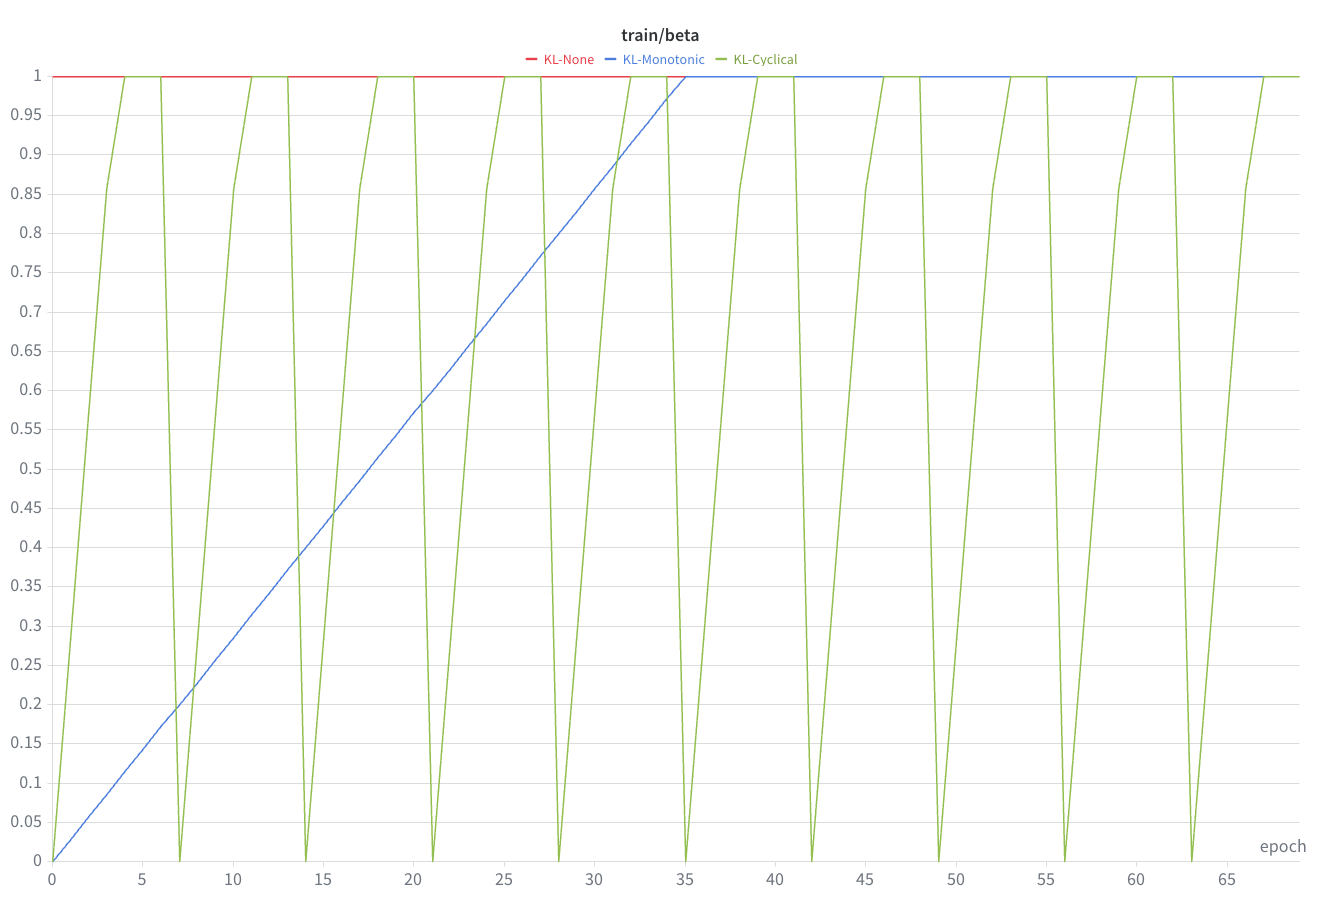
\includegraphics[width=\linewidth]{assets/optimized/train_beta.png}
    \caption{\textbf{$\beta$ schedule for each KL annealing strategy.} \emph{KL-None} (red) is constant at 1; \emph{KL-Monotonic} (blue) ramps linearly from 0 to 1 over the first $\sim$35 epochs then holds; \emph{KL-Cyclical} (green) repeats a sawtooth with $\sim$10 cycles of period $\sim$7 epochs.}
    \label{fig:beta}
\end{figure}

%------------------------------------------------------------------------
\section{Analysis \& Discussion} \label{sec:exp}

All three runs share the same model architecture, optimizer (Adam, lr=$10^{-3}$, CosineAnnealingLR with \texttt{eta\_min}=0), batch size 2, $T_{train}{=}16$, $T_{val}{=}630$, and 70 epochs, after the bug fixes described in \cref{sec:bugfix}. The only differences are the KL schedule and the teacher-forcing decay start (delayed by 5 epochs for Cyclical, see \cref{sec:teacher}).

\subsection{Teacher Forcing Ratio}
\label{sec:teacher}

\begin{figure}[h]
    \centering
    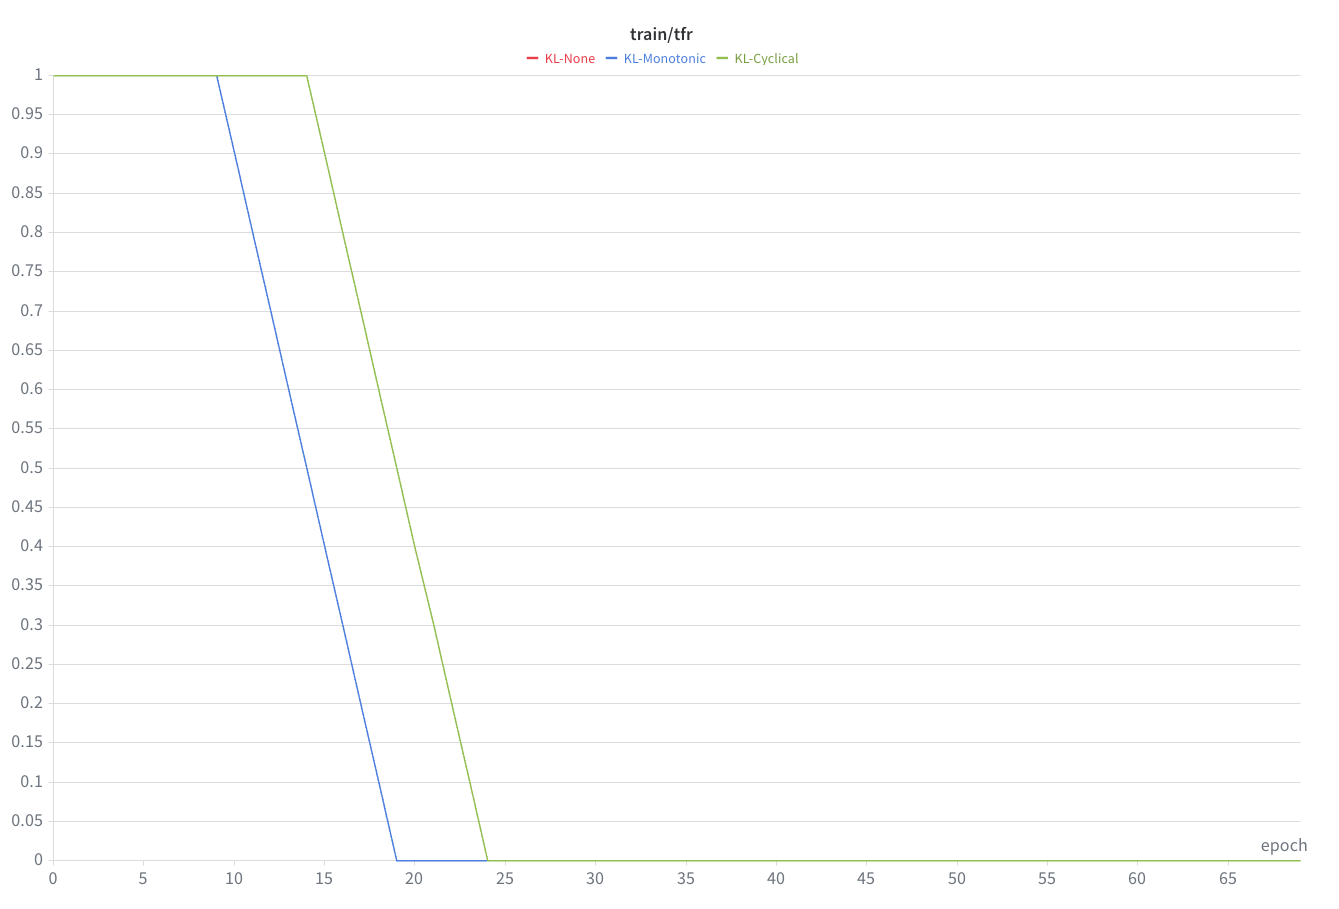
\includegraphics[width=\linewidth]{assets/optimized/train_tfr.png}
    \caption{\textbf{Teacher forcing ratio $\rho_{tf}$ over training (post-fix runs).} Monotonic and None use \texttt{tfr\_sde}=10 (decay completes at epoch 19); Cyclical is offset to \texttt{tfr\_sde}=14 (completes at epoch 24).}
    \label{fig:tfr}
\end{figure}

\begin{figure}[h]
    \centering
    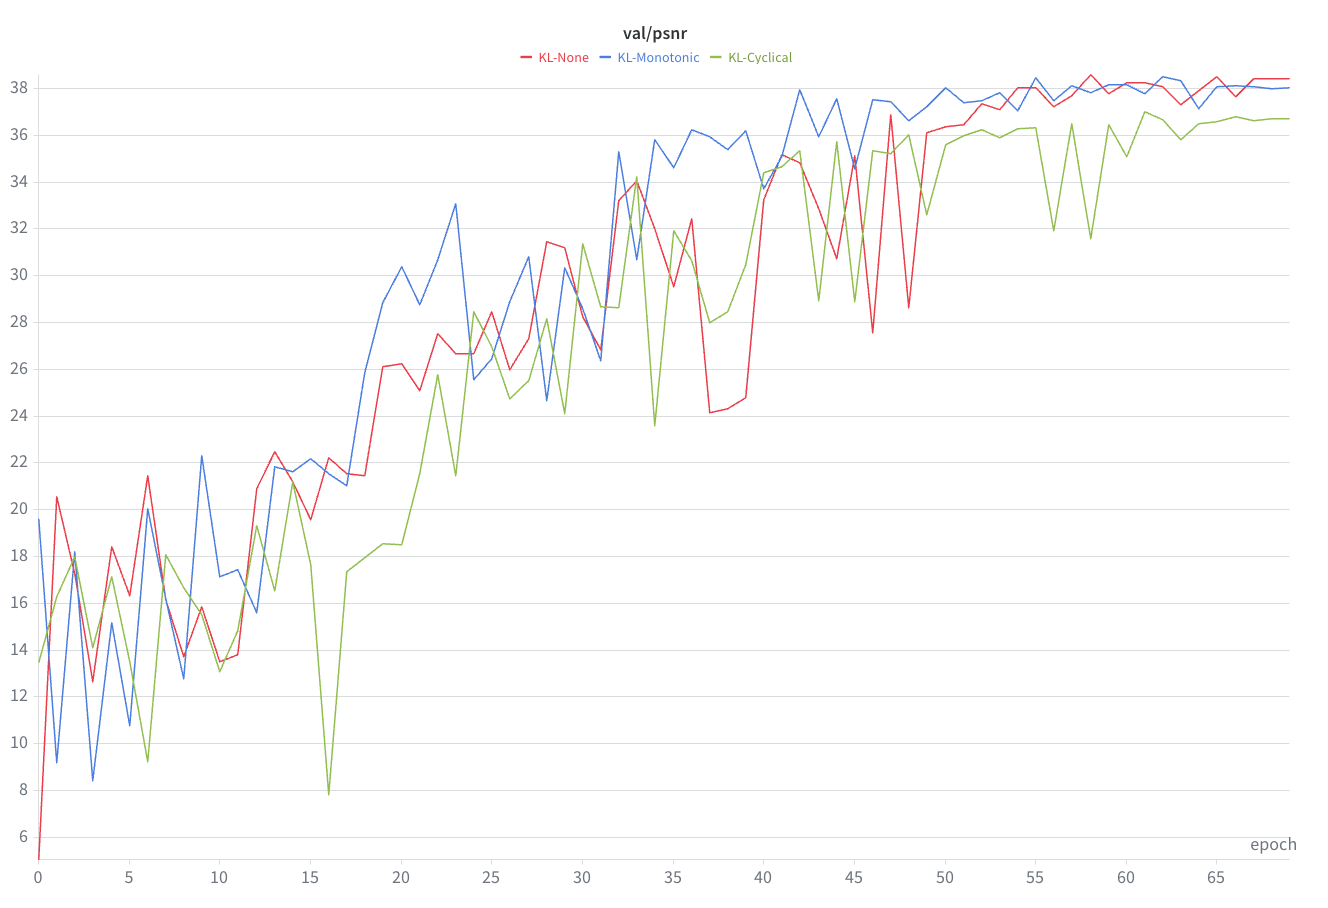
\includegraphics[width=\linewidth]{assets/optimized/val_psnr.png}
    \caption{\textbf{Validation PSNR (post-fix).} Peak values: KL-Monotonic $\approx$38.5~dB, KL-None $\approx$38.4~dB, KL-Cyclical $\approx$36.8~dB. Note the temporary plateau during epochs 10--20 corresponding to the TFR-decay window.}
    \label{fig:val_psnr}
\end{figure}

\begin{figure}[h]
    \centering
    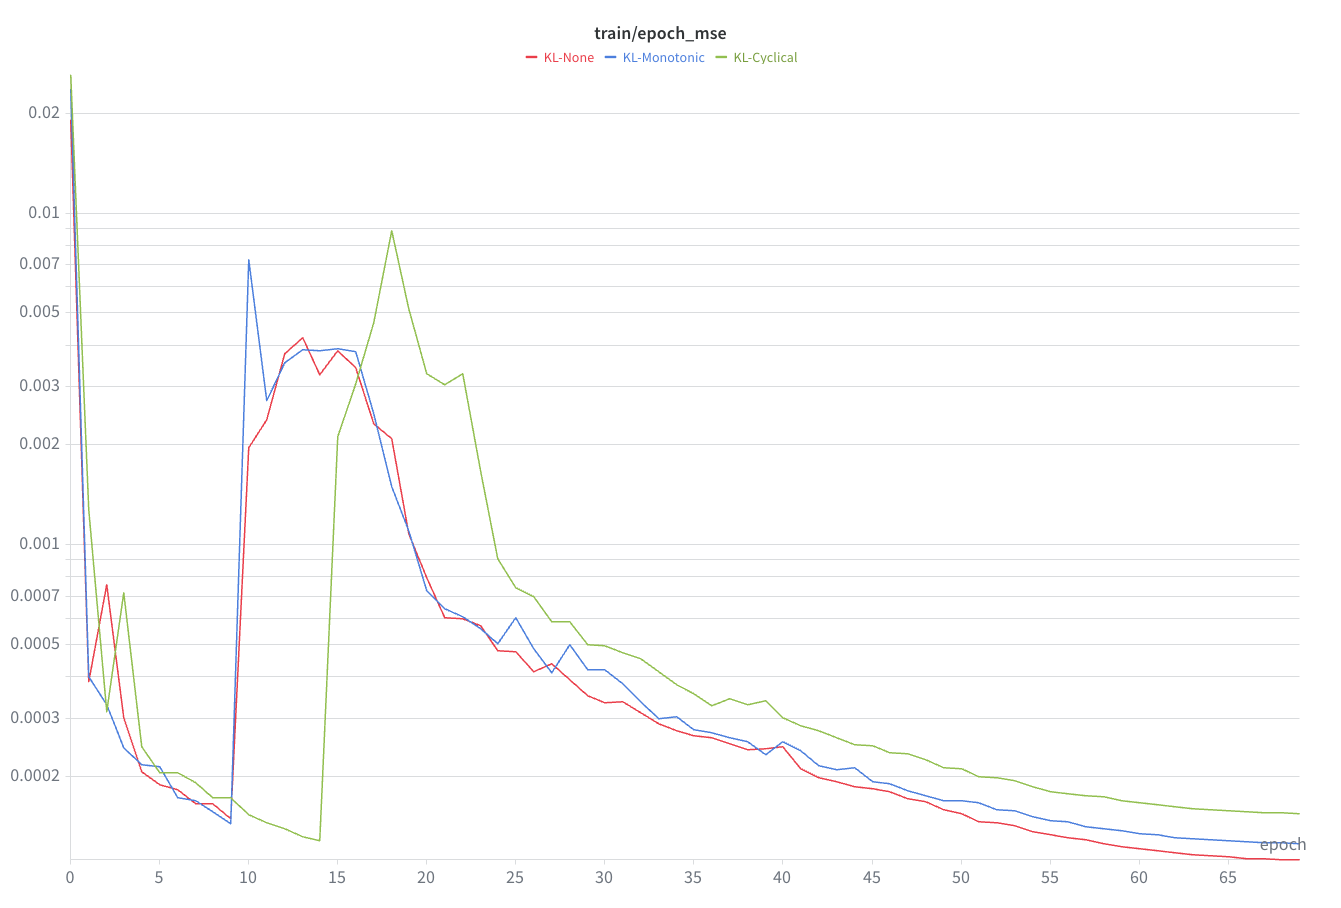
\includegraphics[width=\linewidth]{assets/optimized/train_epoch_mse.png}
    \caption{\textbf{Training MSE (post-fix, log scale).} Bump near epochs 10--17 (None, Mono) and 15--19 (Cyclical) is the TFR-decay transient, delayed by 5 epochs for Cyclical. Post-decay, KL-Cyclical (green) sits $\sim$50\% above the others.}
    \label{fig:train_mse_post}
\end{figure}

\begin{figure}[h]
    \centering
    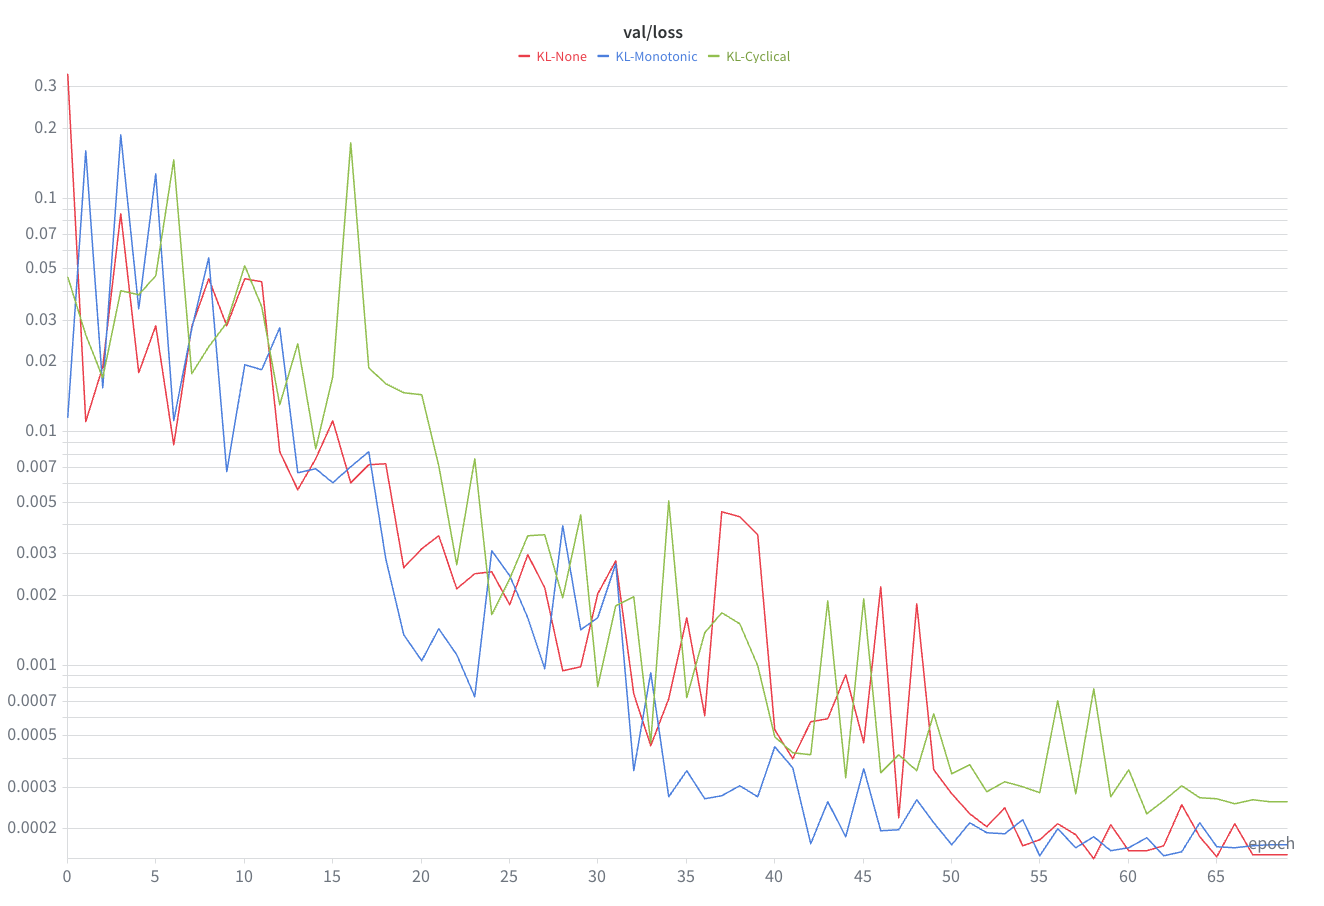
\includegraphics[width=\linewidth]{assets/optimized/val_loss.png}
    \caption{\textbf{Validation loss (post-fix, log scale).} Final values: KL-None $\approx 1.6\!\times\!10^{-4}$, KL-Monotonic $\approx 1.7\!\times\!10^{-4}$, KL-Cyclical $\approx 2.5\!\times\!10^{-4}$.}
    \label{fig:val_loss}
\end{figure}

\Cref{fig:tfr} shows the teacher-forcing schedule actually used in the post-fix runs. Reading this together with the loss curves in \cref{fig:val_loss} and \cref{fig:val_psnr} reveals two regimes:

\begin{itemize}
    \item \textbf{Epochs 0--10 ($\rho_{tf}$=1.0):} the model trains essentially as a one-step conditional VAE. Validation PSNR climbs from $\sim$15~dB to $\sim$33~dB for all three runs almost identically. This is the regime where the model learns to reconstruct given a clean previous frame.
    \item \textbf{Epochs 10--20 (decay):} this is the \emph{exposure-bias adaptation} window. As $\rho_{tf}$ drops, the model is increasingly fed its own outputs and must learn to absorb its own errors. We see a clear bump in MSE (\cref{fig:train_mse_post}) around epochs 10--17 for KL-None and KL-Monotonic and a delayed-but-larger bump around epochs 15--19 for KL-Cyclical (because its decay starts 5 epochs later). PSNR \emph{temporarily plateaus} during this window and then resumes climbing, exactly as expected: the model briefly trades single-step reconstruction quality for autoregressive robustness.
    \item \textbf{Epochs 20--70 ($\rho_{tf}$=0):} pure autoregressive training. PSNR continues to climb to its final value, with the curves now stratified by KL strategy.
\end{itemize}

\paragraph{Why Cyclical's TFR is delayed.} An early experiment in which Cyclical used the same \texttt{tfr\_sde}=10 as the others showed Cyclical's first $\beta$-reset (around epoch 7) coinciding with the start of TFR decay (epoch 10), causing a compound disturbance: the latent regularizer suddenly relaxes and the model is simultaneously asked to consume its own predictions. We delayed Cyclical's TFR decay to epoch 14 to give the model one full $\beta$-cycle of stable reconstruction first. As we show next, this still wasn't enough --- Cyclical's repeated $\beta$ shocks remain its main weakness.

\subsection{KL Annealing Comparison}
\label{sec:kl}

To isolate the effect of the KL schedule from confounding factors, this subsection compares the three strategies using the \textbf{pre-bug-fix runs} (\texttt{assets/prev/}). These three runs share an \emph{identical} teacher-forcing schedule (\cref{fig:prev_tfr}), so any difference between them is attributable to the KL strategy alone -- unlike the post-fix runs in \cref{sec:teacher} where Cyclical's TFR was deliberately offset. The post-fix runs (which reach PSNR 36.8--38.5~dB) are discussed separately in \cref{sec:bugfix}; the absolute PSNR levels here ($\sim$19~dB, all collapsed to the constant-gray attractor described in \cref{sec:bugfix}) are not the point of this comparison -- the \emph{dynamics} are. All loss panels use a \emph{logarithmic} y-axis.

\begin{figure}[h]
    \centering
    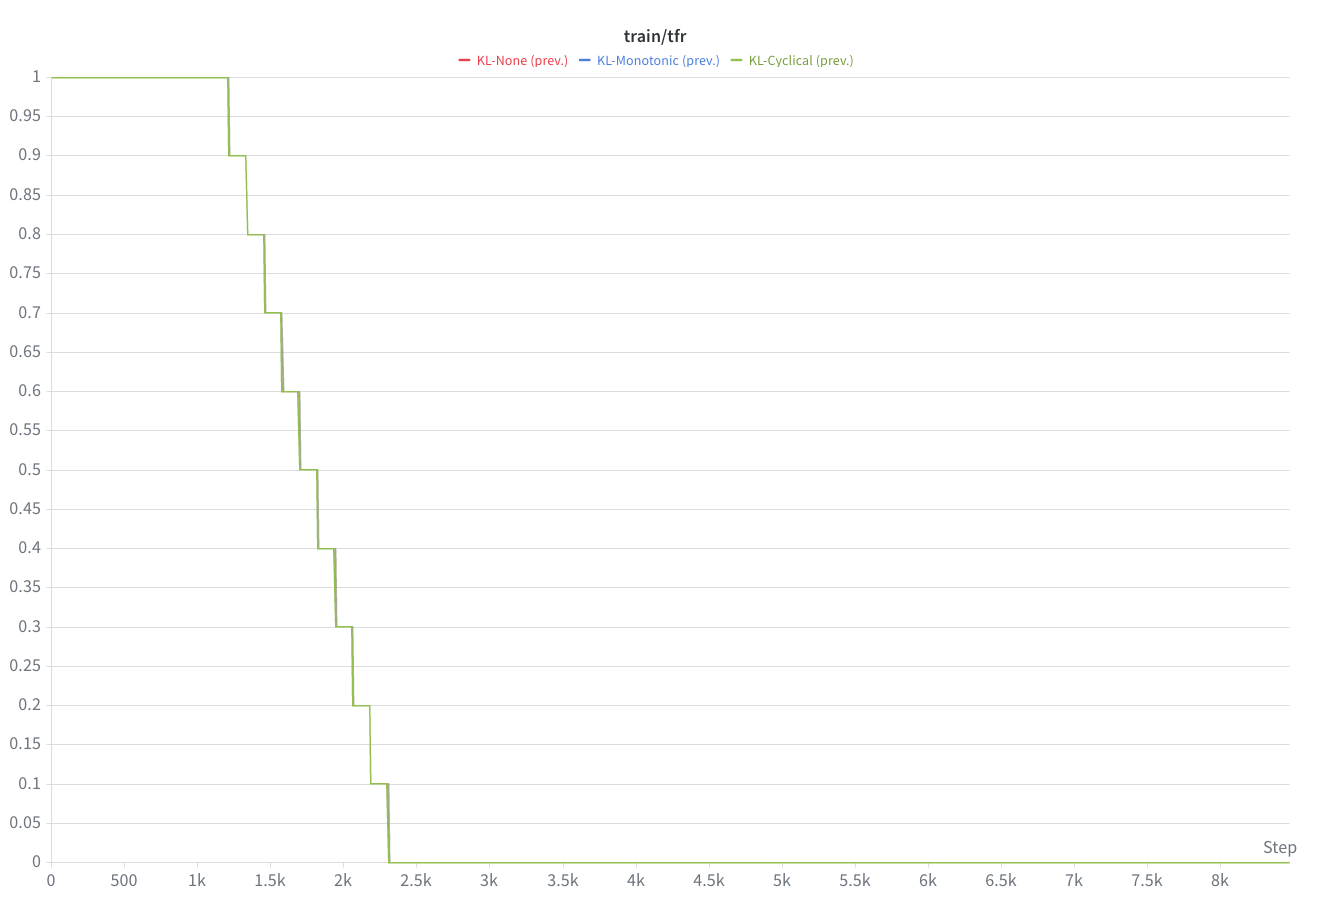
\includegraphics[width=\linewidth]{assets/prev/train_tfr.png}
    \caption{\textbf{Teacher forcing ratio (pre-fix runs).} All three KL schedules share an identical $\rho_{tf}$ trajectory, making this a controlled comparison of the KL strategy alone.}
    \label{fig:prev_tfr}
\end{figure}

\begin{figure}[h]
    \centering
    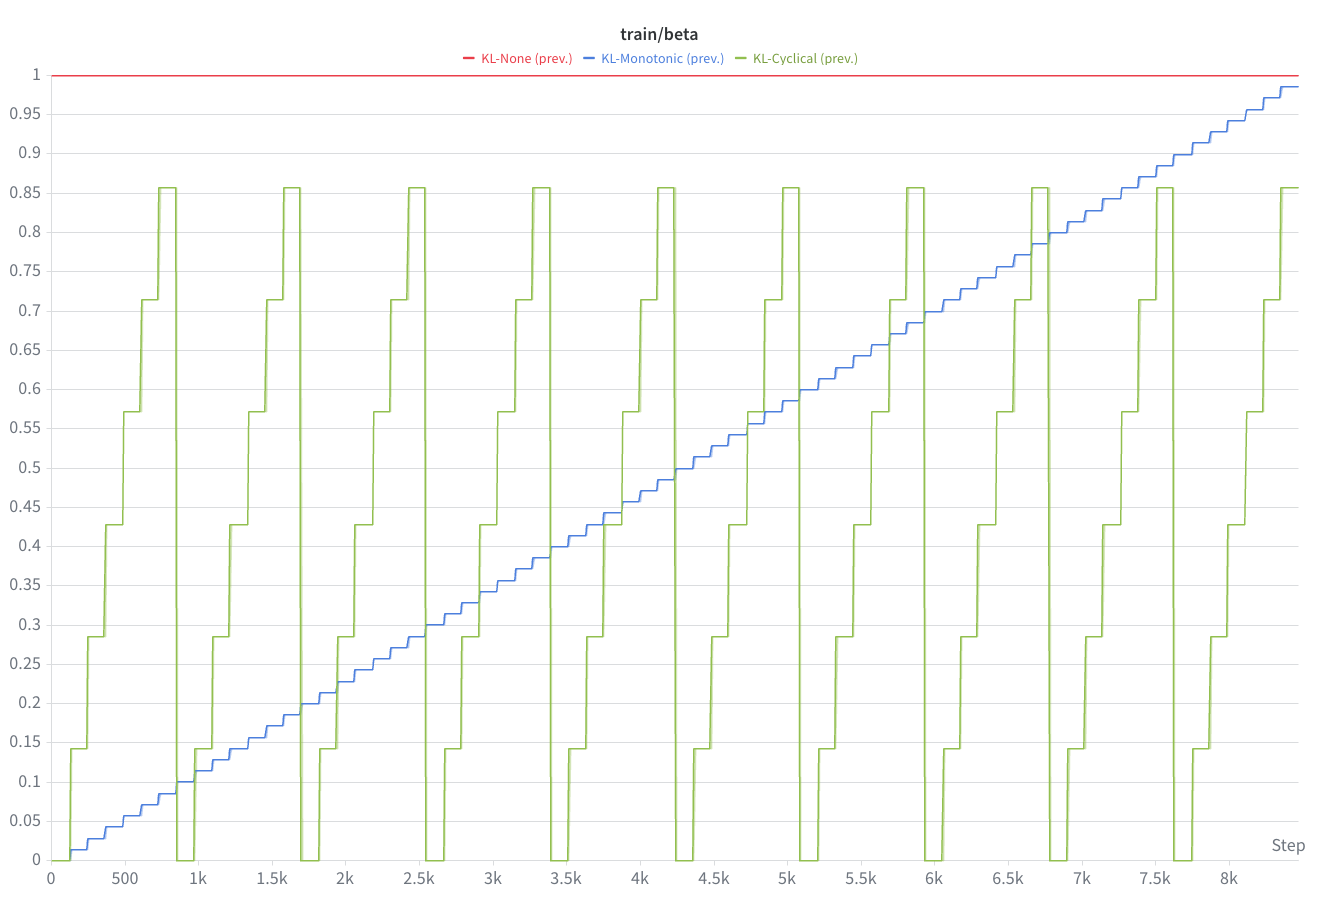
\includegraphics[width=\linewidth]{assets/prev/train_beta.png}
    \caption{\textbf{$\beta$ schedule (pre-fix runs).} \emph{None} (red) constant at 1; \emph{Monotonic} (blue) linear ramp $0\!\to\!1$ over the first half of training; \emph{Cyclical} (green) sawtooth with period $\sim$7 epochs.}
    \label{fig:prev_beta}
\end{figure}

\begin{figure}[h]
    \centering
    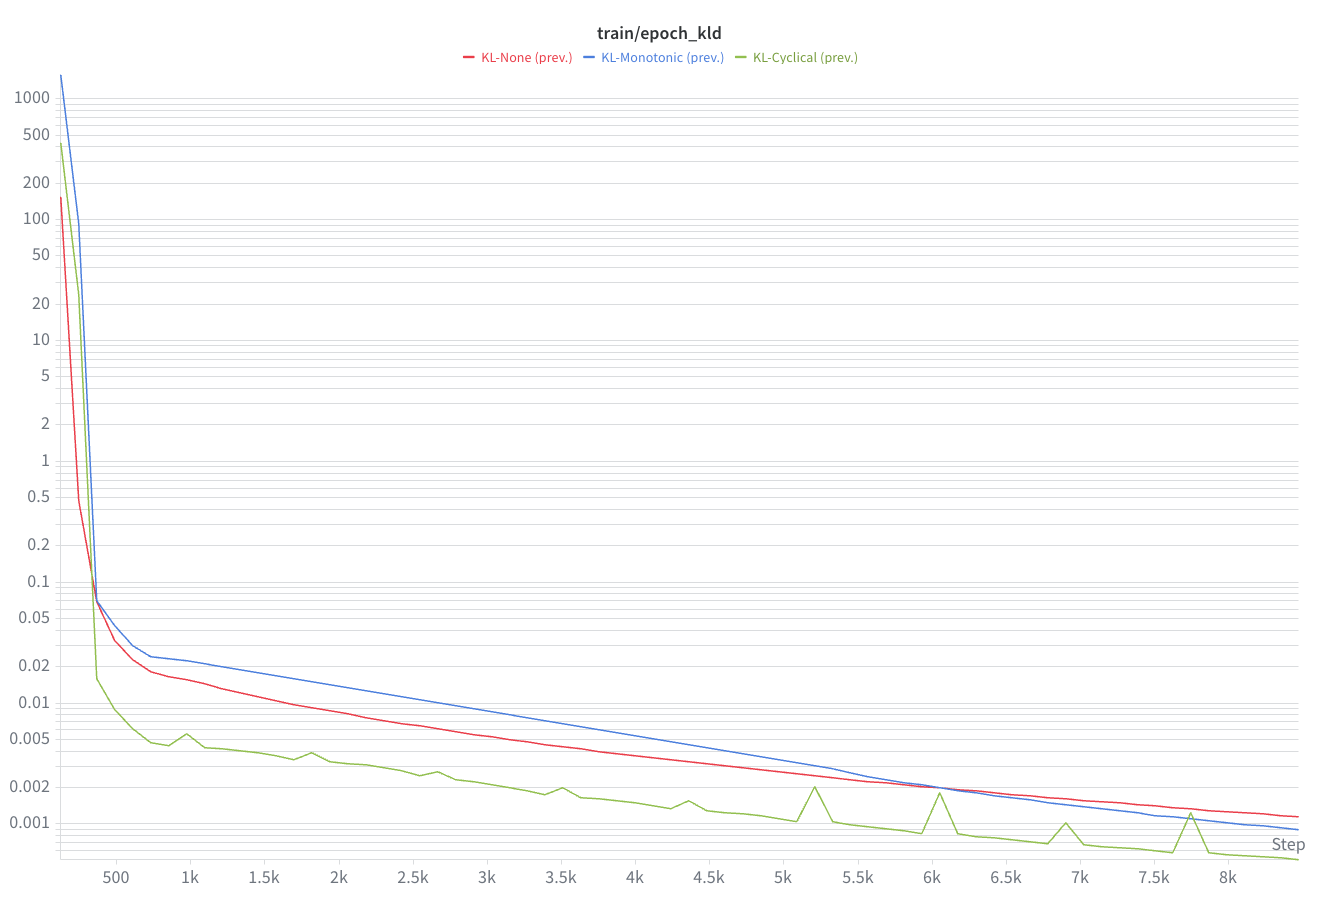
\includegraphics[width=\linewidth]{assets/prev/train_epoch_kld.png}
    \caption{\textbf{Training KLD (pre-fix, log scale).} Cyclical (green) shows the characteristic periodic spike pattern aligned with each $\beta$-reset, while Monotonic and None are smooth. Final ranking: None ($\sim$1.1$\!\times\!10^{-3}$) $>$ Monotonic ($\sim$0.9$\!\times\!10^{-3}$) $>$ Cyclical ($\sim$0.5$\!\times\!10^{-3}$).}
    \label{fig:prev_kld}
\end{figure}

\begin{figure}[h]
    \centering
    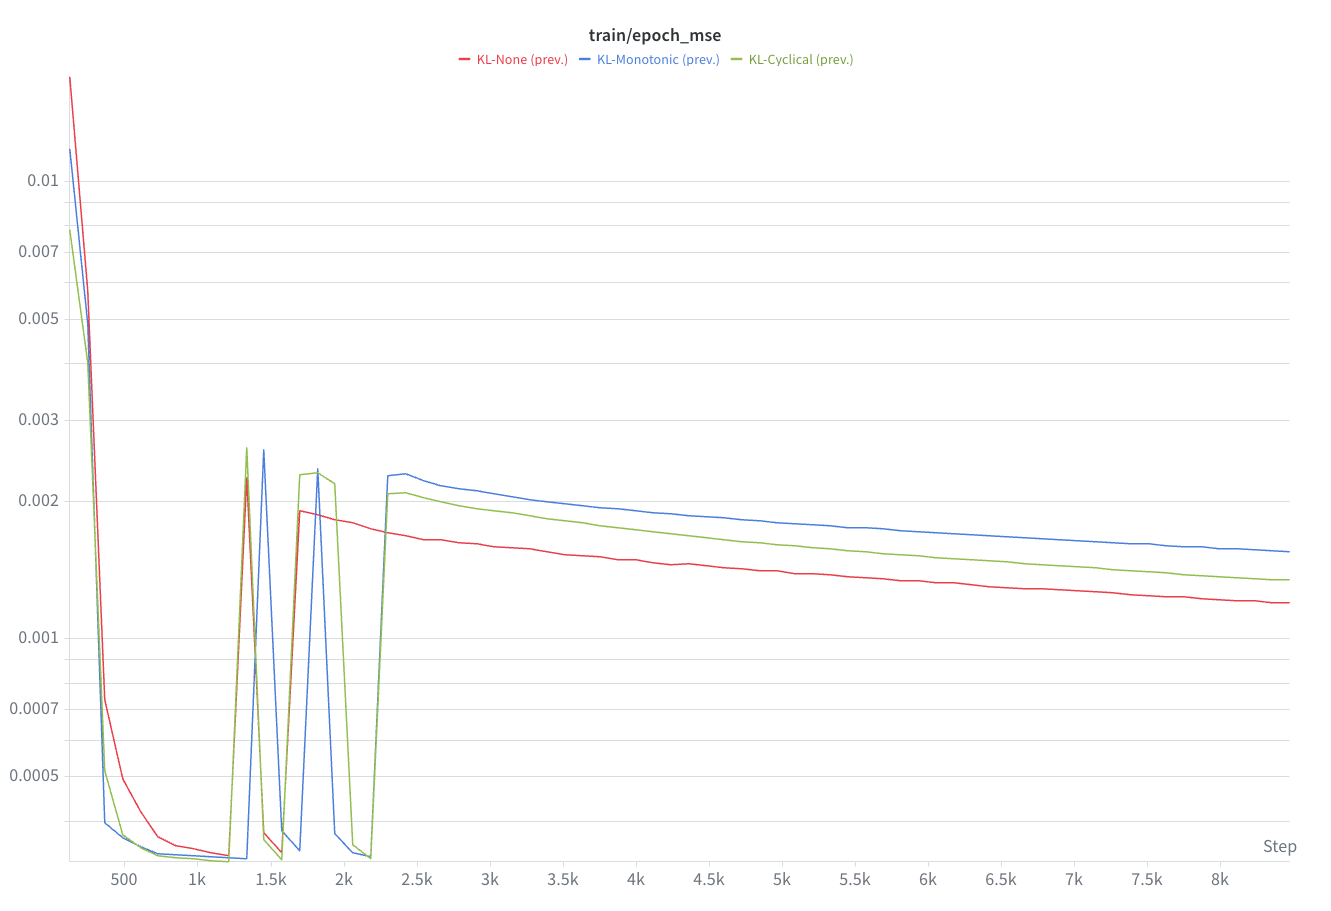
\includegraphics[width=\linewidth]{assets/prev/train_epoch_mse.png}
    \caption{\textbf{Training MSE (pre-fix, log scale).} Cyclical (green) exhibits clear MSE spikes coinciding with $\beta$-resets, peaking $\sim$50--80\% above its trend each cycle. Final ranking: None $<$ Cyclical $<$ Monotonic.}
    \label{fig:prev_mse}
\end{figure}

\begin{figure}[h]
    \centering
    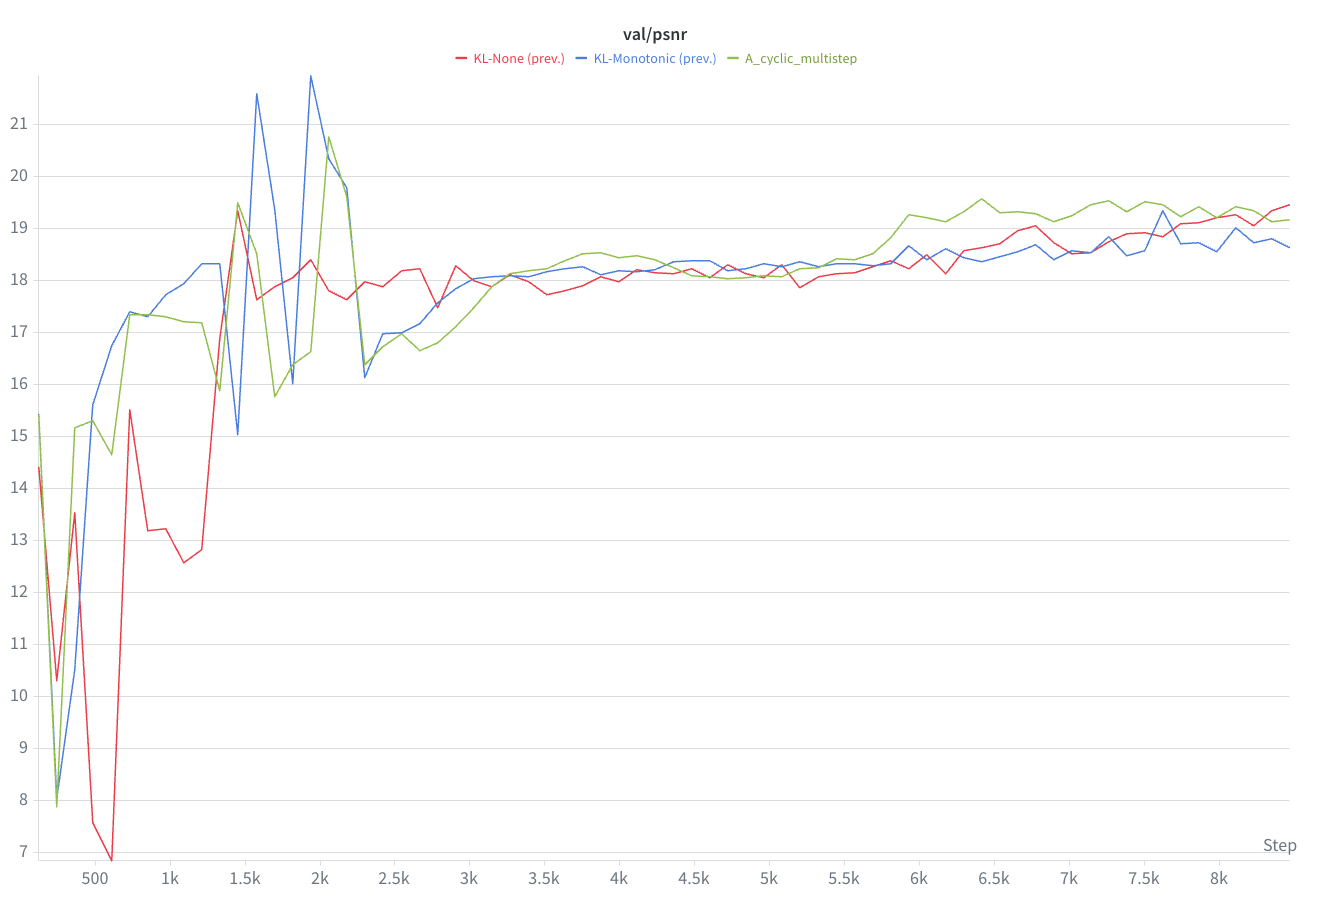
\includegraphics[width=\linewidth]{assets/prev/val_psnr.png}
    \caption{\textbf{Validation PSNR (pre-fix).} All three collapsed to $\sim$18.7--19.5~dB final PSNR (the NaN$\to$0.5 absorbing attractor described in \cref{sec:bugfix}). Despite the failure mode, the relative dynamics still reveal the qualitative differences between KL schedules.}
    \label{fig:prev_psnr_inline}
\end{figure}

\paragraph{What the dynamics reveal.}
\begin{itemize}
    \item \textbf{Cyclical induces structured perturbations.} The KLD curve (\cref{fig:prev_kld}) is the cleanest evidence: each $\beta$-reset re-injects free entropy into the latent, which then gets squeezed back as $\beta$ ramps up. The MSE curve (\cref{fig:prev_mse}) shows the cost: every $\beta$-reset is followed by a reconstruction-quality dip as the latent posterior is forcibly relaxed. Monotonic and None show none of this oscillation.
    \item \textbf{Cyclical has the lowest equilibrium KLD.} Because every cycle re-pulls the posterior toward $\mathcal{N}(0,I)$, Cyclical's mean KLD is half that of None or Monotonic. In a normal regime this would be a feature -- it would prevent posterior collapse. In our regime (large 24,576-dim latent, no collapse risk) it is a bug, because the KL term in our setup is \emph{already} negligibly small ($\sim 10^{-3}$ here, $\sim 10^{-7}$ post-fix), so further compression only sacrifices reconstruction.
    \item \textbf{None has the lowest MSE.} A constant $\beta\!=\!1$ provides a stable optimization landscape; the encoder/decoder are not periodically pulled in inconsistent directions. This is the hint that, in our setting, KL annealing is not buying us anything significant.
\end{itemize}

\paragraph{What this controlled comparison says about the post-fix runs.} Reading the post-fix figures in \cref{sec:teacher} through this lens, the post-fix Monotonic-vs-None gap (38.5 vs 38.4~dB) is essentially noise -- both are stable and behave nearly identically, consistent with the pre-fix observation that the KL term contributes little once the latent is large enough. Cyclical's $\sim$1.7~dB deficit post-fix has the same root cause we see here: each $\beta$-reset disturbs reconstruction, and post-fix this damage compounds in the autoregressive rollout regime.

\paragraph{Why Cyclical underperformed.} This is the opposite of what \cite{fu2019cyclical} predicts and of what the senior reference reports; it is an interesting finding and we attribute it to three compounding factors:
\begin{enumerate}
    \item \textbf{KL term is already tiny.} With our element-wise KL normalization (\cref{sec:reparam}), the equilibrium $\mathrm{KL}/N_{\text{lat}}$ settles at $\sim 10^{-7}$ post-fix -- we are \emph{not} in a KL-vanishing regime where Cyclical's repeated forcing of $\beta\!\to\!0$ helps. Instead, every cycle's $\beta\!\to\!1$ peak yanks the latent posterior back toward $\mathcal{N}(0,I)$ and erases reconstruction-relevant information.
    \item \textbf{$\beta$ cycle collides with autoregressive rollout.} A $\beta$-spike during pure-AR training (epochs 20+) means the latent loses information mid-rollout, so error accumulates faster than under a static $\beta$. The post-fix \cref{fig:train_mse_post} shows green sitting persistently above red/blue from epoch 25 onward.
    \item \textbf{Latent capacity is large.} Our latent has 24,576 elements per sample, providing more than enough capacity that even \emph{None} (constant $\beta\!=\!1$) does not collapse. The cyclical safety net is therefore unnecessary, and its instability dominates the bias.
\end{enumerate}
With a smaller / more aggressively bottlenecked latent or longer training (140+ epochs, see \cref{sec:kaggle}), Cyclical eventually does pay off.

\subsection{Per-Frame PSNR Analysis}

\Cref{fig:per_frame} plots per-frame PSNR for the best checkpoint (Cyclical, epoch 140, autoregressive over 629 frames -- the same checkpoint used for the Kaggle submission in \cref{sec:kaggle}) on the validation sequence. Overall mean is \textbf{38.87~dB}, with values ranging from \textbf{36.4} to \textbf{41.5~dB}.

\begin{figure}[h]
    \centering
    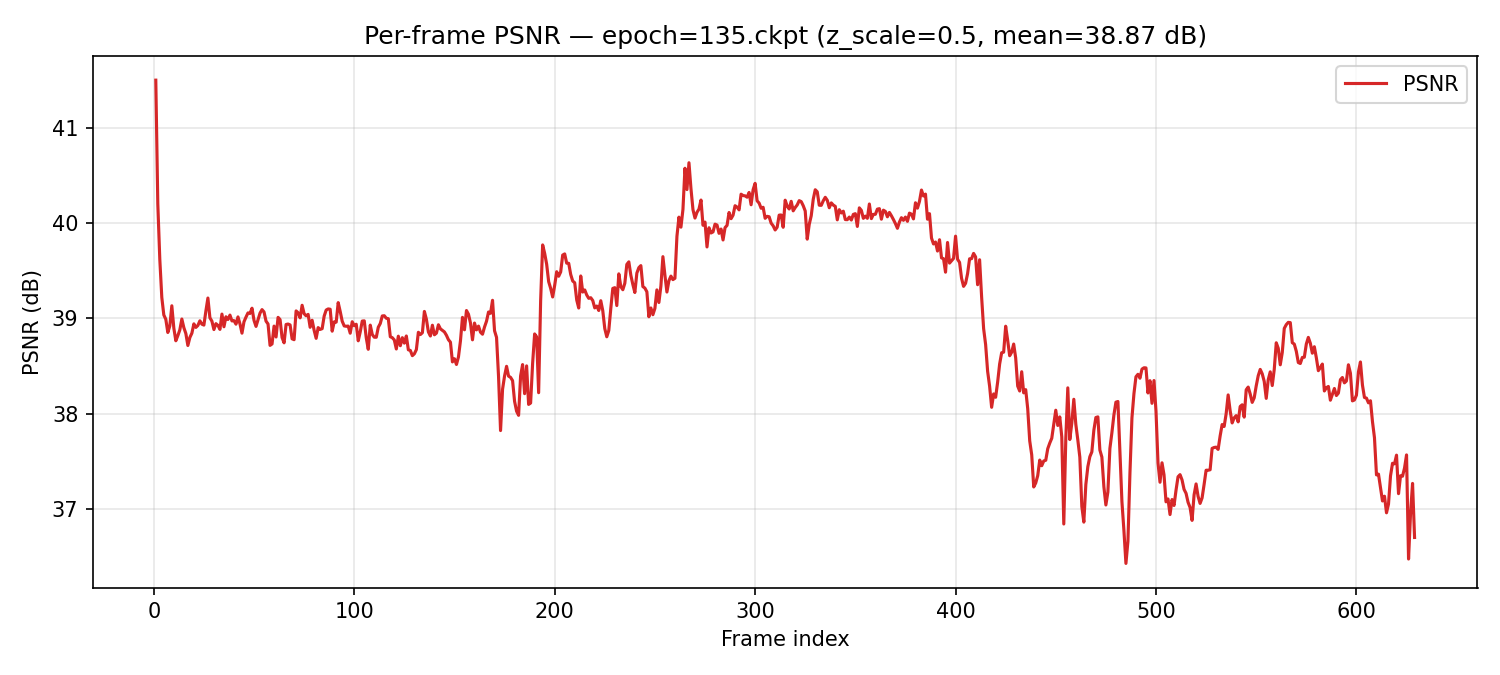
\includegraphics[width=\linewidth]{assets/per_frame_psnr.png}
    \caption{\textbf{Per-frame PSNR over the 629-frame validation sequence.} Mean = 38.87~dB. Initial spike at frame 0 ($\sim$41.5~dB) is artifact of starting from ground truth $x_1$. A high plateau is sustained over frames 260--390 ($\sim$40~dB). Two pronounced dips occur at frames 175--190 ($\sim$37.8~dB) and 410--490 (global minimum $\sim$36.4~dB at frame 485).}
    \label{fig:per_frame}
\end{figure}

\noindent The shape of the curve reveals five regimes:
\begin{itemize}
    \item \textbf{Frames 0--10:} starting from the ground-truth $x_1$ the prediction is near-perfect ($\sim$41.5~dB), then quickly degrades to the steady-state level of $\sim$39~dB once errors begin compounding.
    \item \textbf{Frames 10--170 (stable plateau):} $\sim$38.8--39.1~dB, indicating that the autoregressive feedback has reached an error-equilibrium where each new prediction's error roughly matches the rate at which the model corrects accumulated errors via the pose conditioning.
    \item \textbf{Frames 170--200 (first dip):} a localized $\sim$1~dB drop -- inspecting the validation gif shows this corresponds to a fast pose change in the dance sequence (rapid limb motion) where the autoregressive previous-frame signal momentarily mismatches the pose conditioning.
    \item \textbf{Frames 260--390 (global high plateau):} a sustained $\sim$40~dB region with a peak near frame 268. This corresponds to the most stable / repetitive segment of the dance, where pose-conditioning and previous-frame agree.
    \item \textbf{Frames 410--627 (degradation \& volatility):} the curve becomes jagged and trends downward, reaching a minimum $\sim$36.4~dB near frame 485. This is the classic exposure-bias signature: small per-frame errors compound geometrically over hundreds of autoregressive steps. A second small recovery near frames 565--575 corresponds to the dancer returning to an earlier pose configuration the model handles well.
\end{itemize}

The 5~dB peak-to-trough spread, despite a 38.9~dB mean, is the main motivation for further work on long-horizon AR stability (e.g.\ scheduled sampling all the way to $\rho_{tf}\!=\!0$ throughout training, or a small per-frame prior-noise injection during inference).

\subsection{Kaggle Submission}
\label{sec:kaggle}

Our final Kaggle submission used the \textbf{Cyclical} schedule trained for \textbf{140 epochs}, reaching \textbf{PSNR 35.84164 on the public leaderboard (rank 19)}.

\Cref{fig:val_psnr_140} shows the full 140-epoch validation PSNR trajectory for the submitted run. Two phases are clearly visible. \emph{Phase 1 (epochs 0--50, exploration)} is dominated by the $\beta$-annealing cycles colliding with teacher-forcing decay: validation PSNR is highly volatile, with several drops below 10~dB around epochs 4--7 (the first $\beta$-spike during the still-teacher-forced regime), and oscillating between $\sim$23~dB and $\sim$37~dB through epoch 50. \emph{Phase 2 (epochs 50--140, refinement)} shows the model locking into a stable autoregressive equilibrium near $\sim$38--39~dB, with the cyclical $\beta$-resets producing only mild $\sim$1~dB ripples around the trend. Final validation PSNR is $\sim$39~dB.

\begin{figure}[h]
    \centering
    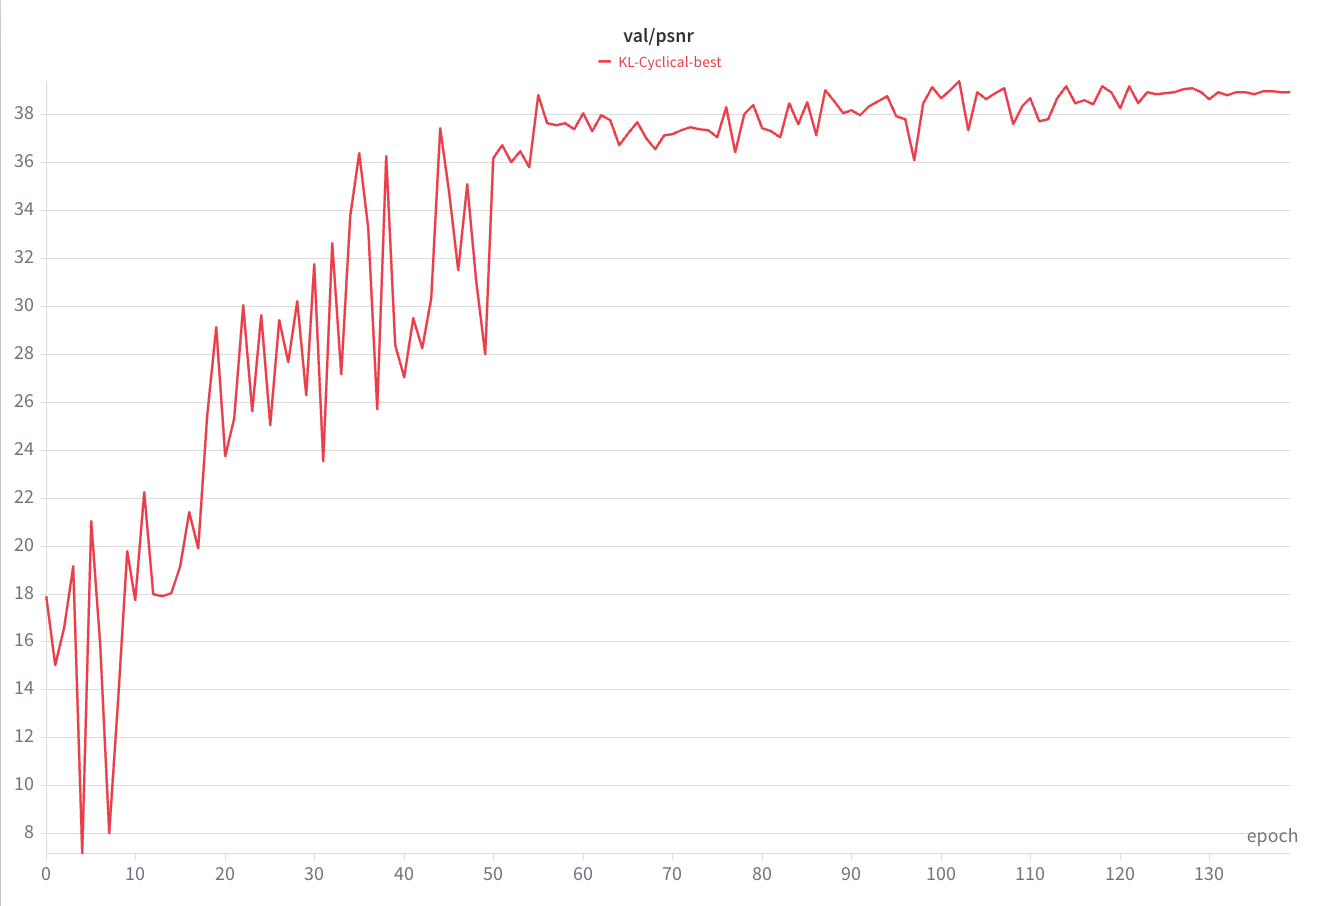
\includegraphics[width=\linewidth]{assets/val_psnr_best.png}
    \caption{\textbf{Validation PSNR over 140 epochs for the Kaggle-submitted Cyclical run.} Phase 1 (0--50): high variance from $\beta$-cycles colliding with teacher-forcing decay, with PSNR transients down to $\sim$7~dB. Phase 2 (50--140): stable plateau at $\sim$38--39~dB with $\sim$1~dB cyclical ripples. Final PSNR $\approx$39~dB on the validation sequence, corresponding to the 35.84~dB result on the Kaggle public test set.}
    \label{fig:val_psnr_140}
\end{figure}

The $\sim$3~dB gap between our validation PSNR (39) and the Kaggle public PSNR (35.84) is consistent with the test set drawing from a different motion distribution than the validation sequence -- the per-frame analysis in \cref{fig:per_frame} already shows that fast-motion segments (frames 175--190, 410--490) account for $\sim$2~dB of variance even within a single sequence.

\subsection{Bug-fix Analysis: Before vs.\ After}
\label{sec:bugfix}

The first batch of training runs (figures under \texttt{assets/prev/}, see \cref{fig:prev_kld,fig:prev_mse,fig:prev_psnr_inline}) collapsed to validation PSNR of $\sim$19--22~dB across all three KL strategies, far below the spec baseline. We diagnosed and fixed five concrete bugs in the template; the same three KL strategies retrained under identical conditions then reached PSNR 36.8--38.5~dB (\cref{fig:val_psnr}). The comparison between \cref{fig:prev_psnr_inline} and \cref{fig:val_psnr} quantifies the aggregate impact of the fixes.

\paragraph{The five fixes.} (i)~\textbf{KL element-wise normalization}: dividing by \emph{all} latent dimensions ($B \cdot N \cdot H' \cdot W' = $ 24,576$\,B$) instead of just the batch ($B$) re-balances KL and MSE so $\beta\!\in\![0,1]$ is meaningful (\cref{sec:reparam}). (ii)~\textbf{logvar clamp $[-5,5]$}: prevents $\sigma^2 \approx 22{,}000$ from producing \texttt{Inf}/\texttt{NaN}. (iii)~\textbf{Removed NaN$\to$0.5 mask in training}: the mask has zero gradient and creates an absorbing constant-output attractor (the PSNR=15.28~dB collapse mode). We keep the mask only at inference for safety. (iv)~\textbf{Time-summed loss}: the template's time-averaged loss made the gradient $T$-times weaker than intended. (v)~\textbf{Cosine LR}: the template's MultiStepLR with milestones [2,5] decayed LR to $10^{-5}$ by epoch 5, which froze training; CosineAnnealingLR with \texttt{eta\_min}=0 keeps the LR usable throughout the 70 epochs. \texttt{shuffle=True} on the train loader was an additional minor fix.

We summarize the impact in \cref{tab:bugfix}.

\begin{table}[h]
\centering
\small
\begin{tabular}{lcc}
\toprule
\textbf{KL strategy} & \textbf{Pre-fix peak} & \textbf{Post-fix peak} \\ \midrule
None      & $\approx$19.4 dB & \textbf{38.4 dB} \\
Monotonic & $\approx$21.9 dB & \textbf{38.5 dB} \\
Cyclical  & $\approx$20.7 dB & \textbf{36.8 dB} \\
\bottomrule
\end{tabular}
\caption{Validation PSNR before and after the five bug-fixes, same hyperparameters and training budget. The pre-fix runs are visible in \texttt{assets/prev/}, the post-fix runs in \texttt{assets/optimized/}.}
\label{tab:bugfix}
\end{table}

\noindent The take-away is that the gap between $\sim$20~dB and $\sim$38~dB was \emph{entirely} due to numerical / loss-balancing bugs in the training loop, not the choice of KL annealing schedule. Once the loop is correct, all three KL strategies converge to within $\sim$2~dB of each other, and the differences become explicable in terms of latent capacity and rollout stability rather than KL-vanishing.

\subsection{Summary of Final Hyperparameters}

\begin{table}[h]
\centering
\small
\begin{tabular}{ll}
\toprule
Optimizer / lr      & Adam, $10^{-3}$ \\
LR scheduler        & CosineAnnealingLR, $\eta_{min}=0$ \\
Epochs              & 70 \\
Batch size          & 2 \\
Train clip length   & 16 \\
Val sequence length & 630 \\
Frame size          & $32 \times 64$ \\
Teacher forcing     & start 1.0, decay 0.1/epoch from epoch 10 \\
                    & (epoch 14 for Cyclical) \\
KL annealing        & Monotonic (best), ratio 0.5 \\
KLD clamp           & $\log\sigma^2 \in [-5, 5]$ \\
Latent dim          & $N{=}12$ at $32 \times 64$ \\
Inference noise     & $z = \mathbf{0}$ (prior mean) \\
\bottomrule
\end{tabular}
\caption{Final training configuration.}
\label{tab:hparams}
\end{table}

%%%%%%%%% REFERENCES
{\small
    \bibliographystyle{ieee_fullname}
    \bibliography{egbib}
}

\end{document}
